\chapter{Results}

\section{Hardware testing}

A total of 40 FLX-182-1B cards, in 3 different batches, were subjected hardware validation and testing. During this process, 10 cards were found to be non-functional due to a range of issues, including component failures and configuration errors. Through the aformentioned diagnostics and interventions, 8 of the faulty cards were fully or partially recovered and restored to operational status.\\
All the recovered cards are now delivered to the institutes and functioning properly.

\section{Performance measurements: netio3}
\label{sec:netio3-perf}
The network performance evaluation focused on two key parameters: Throughput and \ac{RTT}. The experiments were conducted in a controlled testbed environment using servers connected via a 200 Gbit/s Ethernet link through a switch. The hardware specifications of the servers are detailed below:

\clearpage
\begin{lstlisting}[caption={Network interface information}, label={lst:network}]
[mshehu@pc-tbed-felix-15 ~]$ lspci | grep -E -i --color 'network|ethernet'
41:00.0 Ethernet controller: Mellanox Technologies MT2910 Family [ConnectX-7]
41:00.1 Ethernet controller: Mellanox Technologies MT2910 Family [ConnectX-7]
81:00.0 Ethernet controller: Intel Corporation Ethernet Controller X550 (rev 01)
81:00.1 Ethernet controller: Intel Corporation Ethernet Controller X550 (rev 01)
\end{lstlisting}

\begin{lstlisting}[caption={CPU information}, label={lst:cpu}, float=htbp]
[mshehu@pc-tbed-felix-15 ~]$ lscpu
Architecture:             x86_64
  CPU op-mode(s):         32-bit, 64-bit
  Address sizes:          52 bits physical, 57 bits virtual
  Byte Order:             Little Endian
CPU(s):                   64
  On-line CPU(s) list:    0-63
Vendor ID:                AuthenticAMD
  Model name:             AMD EPYC 9354P 32-Core Processor
    CPU family:           25
    Model:                17
    Thread(s) per core:   2
    Core(s) per socket:   32
    CPU max MHz:          3799.0720
    CPU min MHz:          1500.0000
\end{lstlisting}

\begin{lstlisting}[caption={Memory information}, label={lst:memory}]
[mshehu@pc-tbed-felix-15 ~]$ lsmem
RANGE                                 SIZE  STATE REMOVABLE BLOCK
0x0000000000000000-0x000000187fffffff  98G online       yes  0-48
\end{lstlisting}

Statics have been collected from the sending part; the reason was because the sending part interrupts the connection, and the statistics collection could be stopped at the same time.

\subsection{Throughput}

The throughput tests were conducted using the two \textit{netio3-backends} LIBFABRIC-RDMA and ASYNCMSG-TCP. To manage the high number of tests, an Ansible \cite{ansible} playbook was developed. The output of the playbook was processed using a custom Python script, which also generated the graphs using the Matplotlib \cite{matplotlib} library. The tests involved varying the buffer size --- ranging from 1 KB to 64 KB  (in ATLAS production are used buffers of 64 KB) --- and the number of buffers. The same buffer size and number of buffers were used for both the sender and receiver. 

The sender transmits buffers sequentially, employing a polling mechanism to determine when the next buffer could be sent. The receiver, in turn, simply ackowledges and discards the incoming messages without further processing, as the primary objective was to measure throughput. A total of 70 combinations of buffer sizes and counts were tested for LIBFABRIC-RDMA, while only 28 combinations were evaluated for ASYNCMSG-TCP due to diminishing returns observed in preliminary tests.

\subsubsection{Analysis}

Figures \ref{fig:1kb-buffer-throughput} and \ref{fig:64kb-buffer-throughput} show the LIBFABRIC-RDMA backend measurements for the two extreme cases: a 1 KB buffer and a 64 KB buffer.

\begin{figure}[htbp]
\centering
\begin{subfigure}[b]{0.7\textwidth}
    \centering
    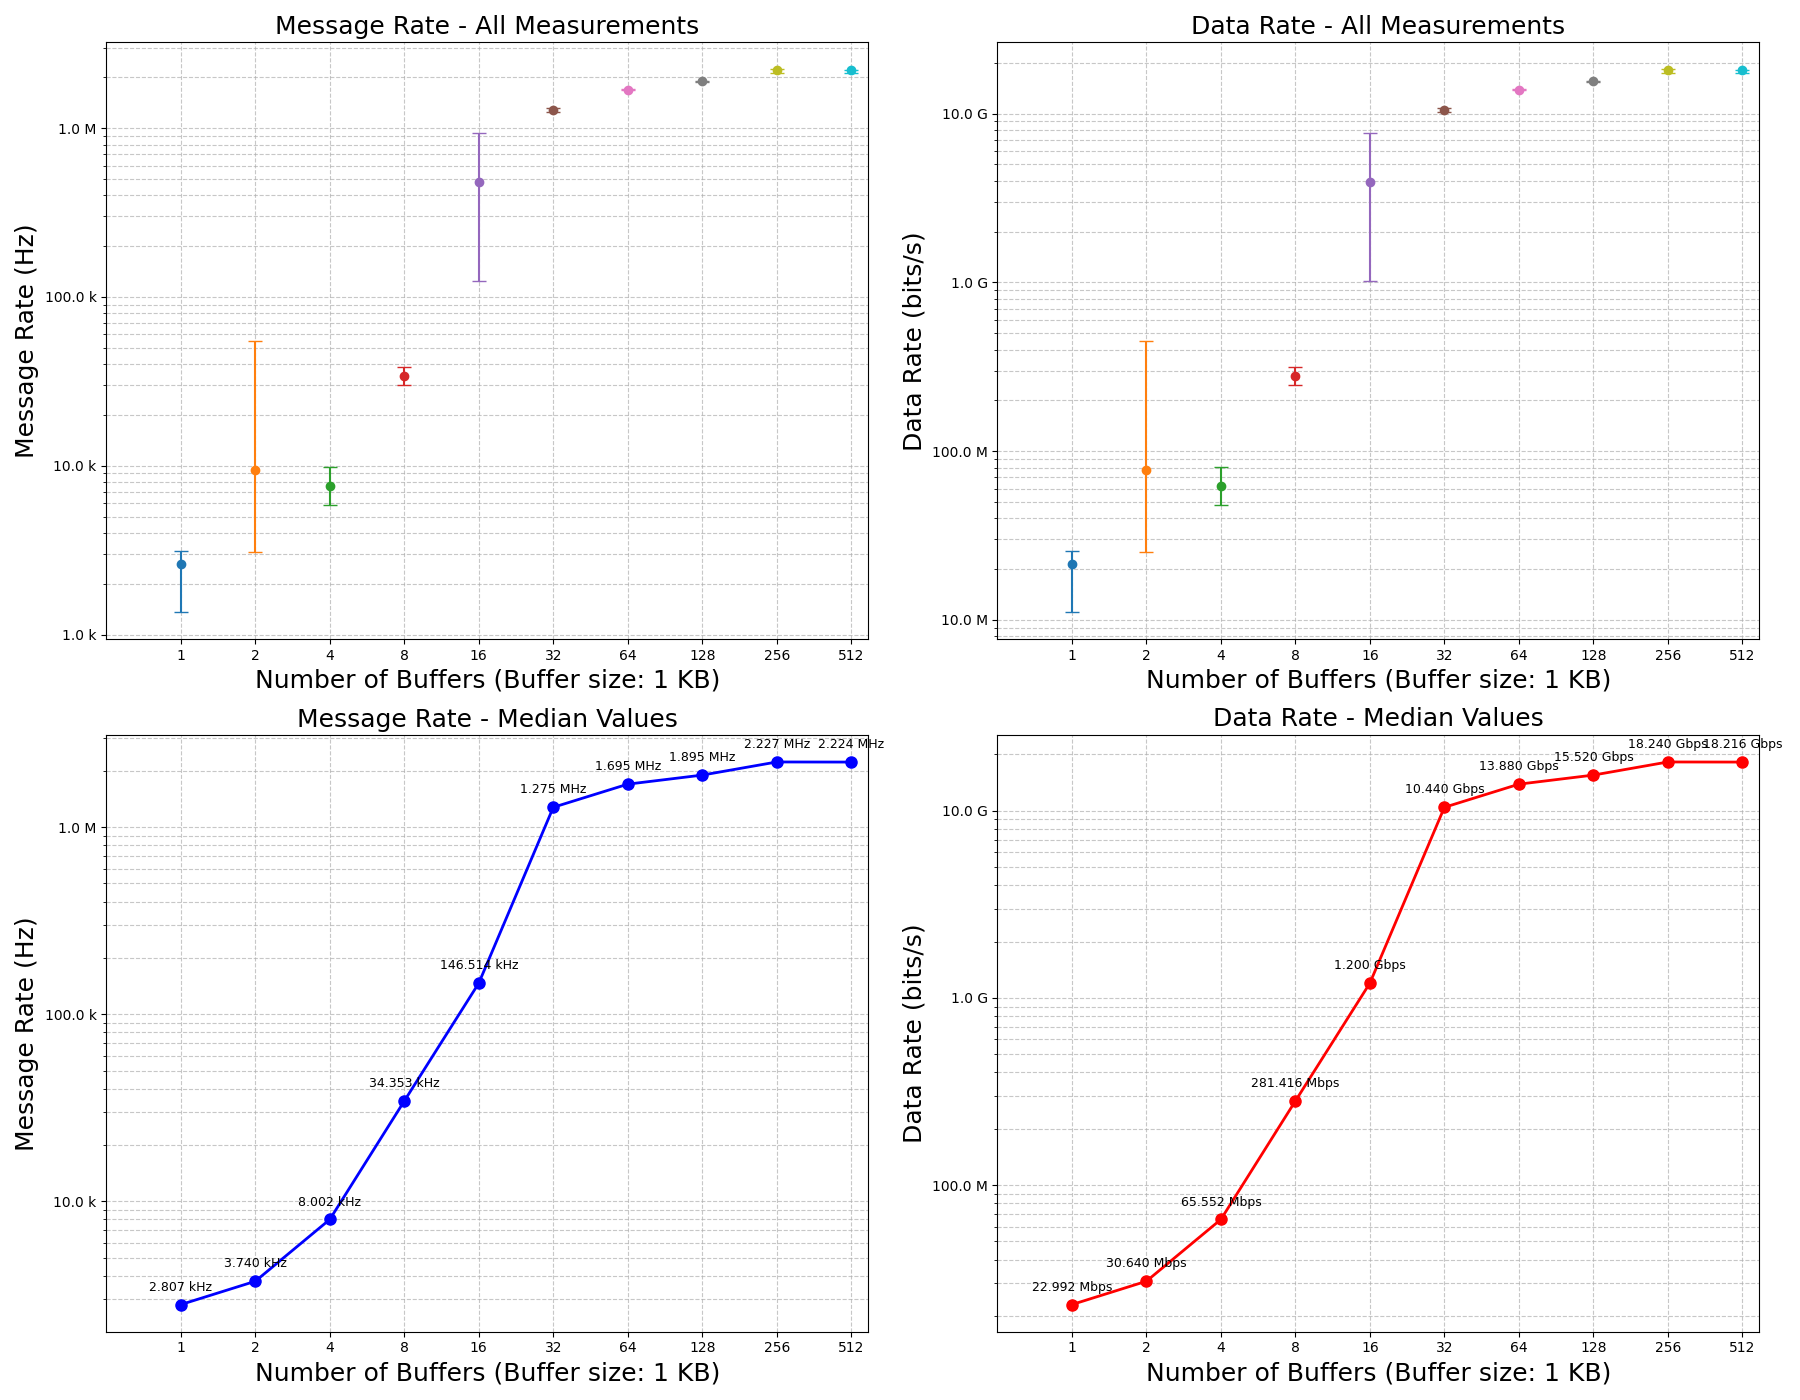
\includegraphics[width=\textwidth]{images/results/libfabric_throughput_analysis_1K.png}
    \caption[Network performance with a 1 KB buffer]{Network performance with a 1 KB buffer. \textbf{Left:} message frequency, \textbf{Right:} Data Throughput. \textbf{Top:} plots with error ranges, \textbf{Bottom:} median values.}
    \label{fig:1kb-buffer-throughput}
\end{subfigure}
\vspace{0.2cm}
\begin{subfigure}[b]{0.7\textwidth}
    \centering
    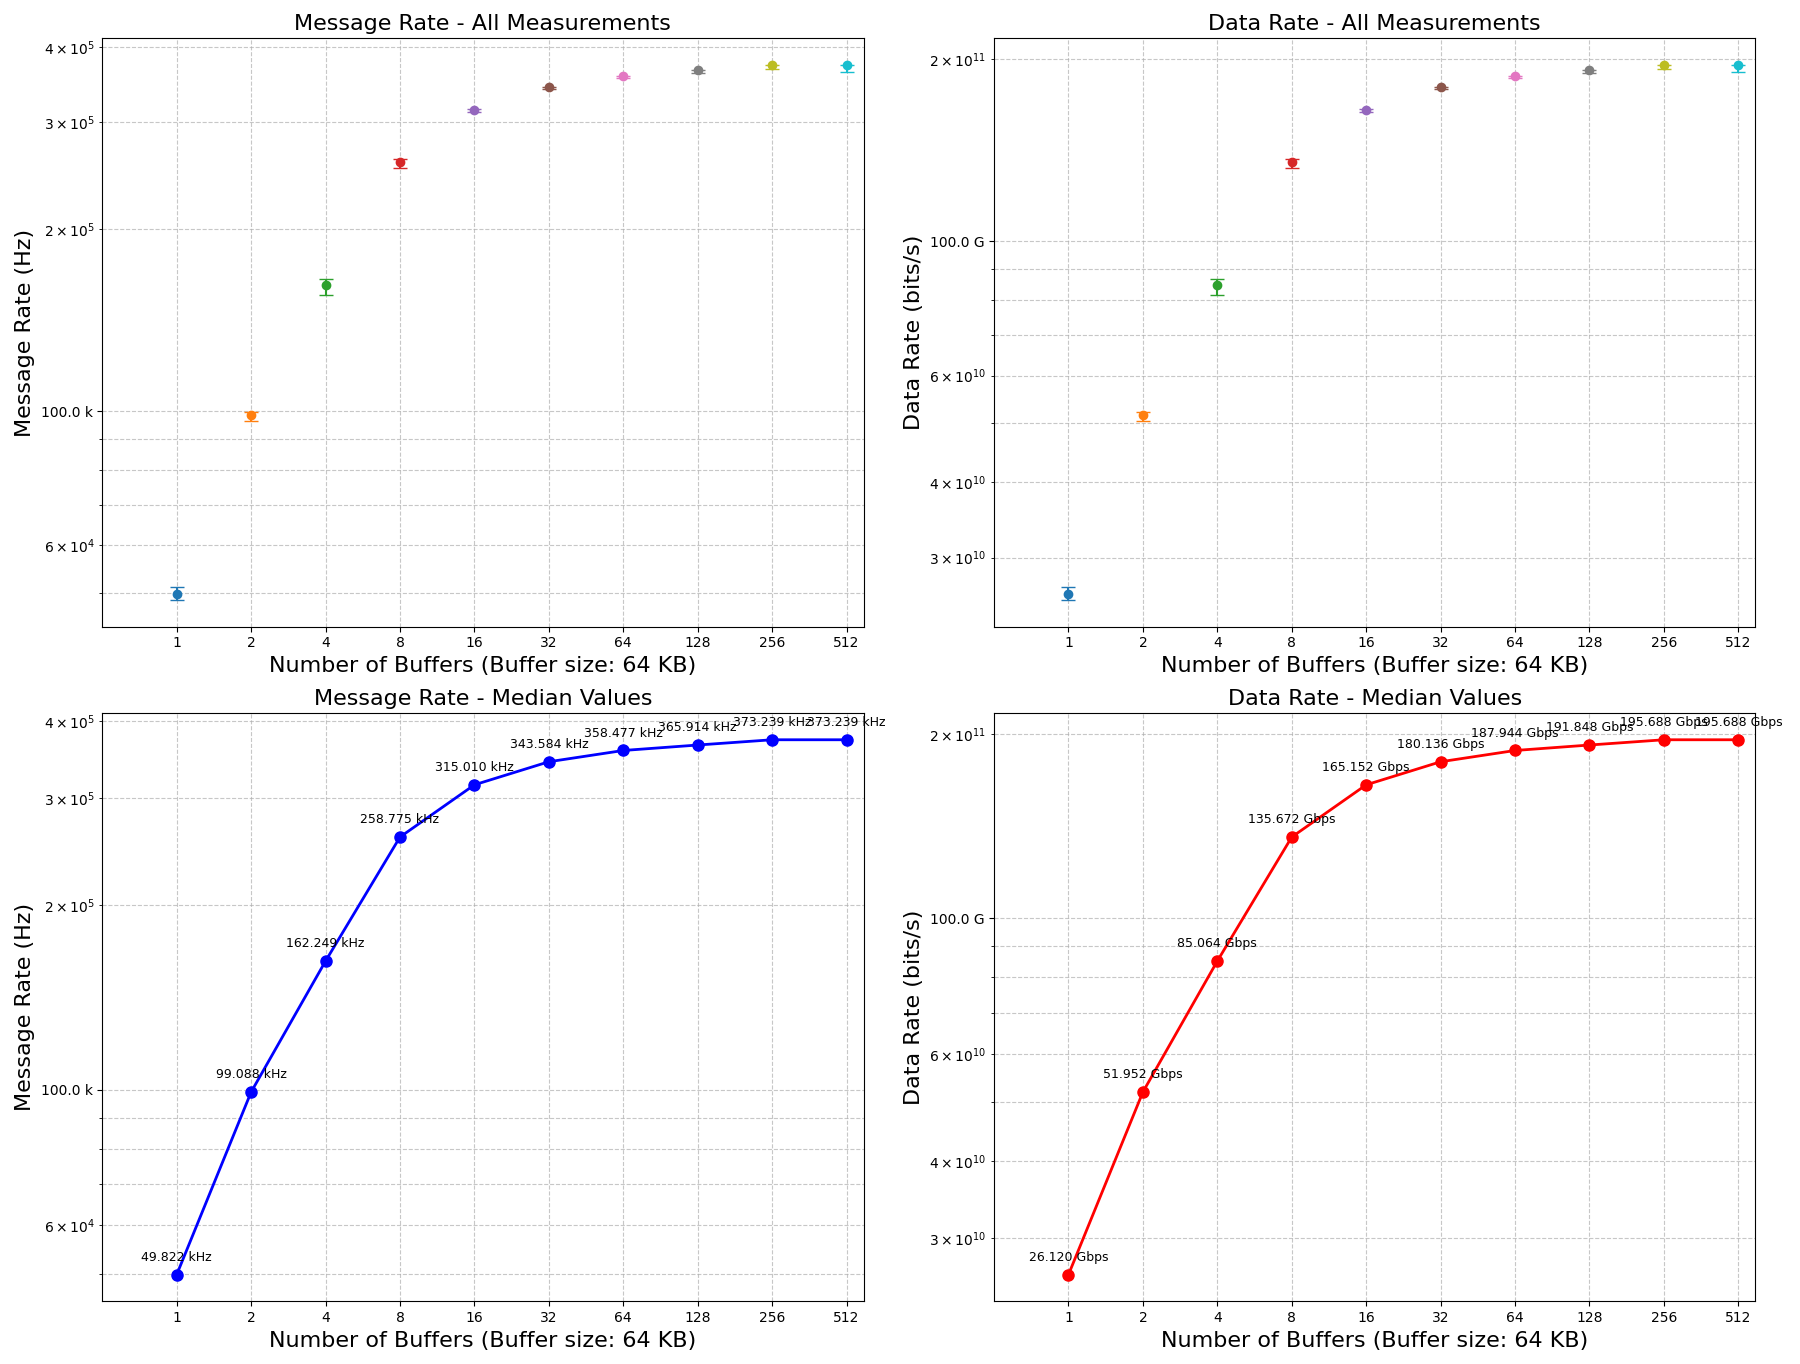
\includegraphics[width=\textwidth]{images/results/libfabric_throughput_analysis_64K.png}
    \caption[Network performance with a 64 KB buffer]{Network performance with a 64 KB buffer. \textbf{Left:} message frequency, \textbf{Right:} Data Throughput. \textbf{Top:} plots with error ranges, \textbf{Bottom:} median values.}
    \label{fig:64kb-buffer-throughput}
\end{subfigure}
\caption[Throughput comparison of 1KB and 64KB buffer]{The error rate of the smaller 1KB buffers is relatively high, while for the 64KB buffers the effect is much more contained.}
\label{fig:throughput-of-the-extremes-1K-64K}
\end{figure}

The results indicate that smaller buffers (e.g., 1 KB) exhibit a large variation of throughput due to the overhead associated with connection establishment, which is significant relative to the transmission time for small messages. In contrast, larger buffers (e.g., 64 KB) exhibit a small variance, as the connection overhead becomes negligible compared to the transmission time.

To mitigate the impact of these variations (especially for smaller buffers), the median throughput was used for comparison.

Figure \ref{fig:libfabric-mean-throughput-comparison} presents the throughput comparison for LIBFABRIC-RDMA across all buffer sizes. The results highlight that buffers smaller than 8 KB and a fewer number of buffers than 16 should be avoided if the goal is maximum throughput. For larger buffers, the behavior aligns with expectations. 

\begin{figure}[htbp]
\centering
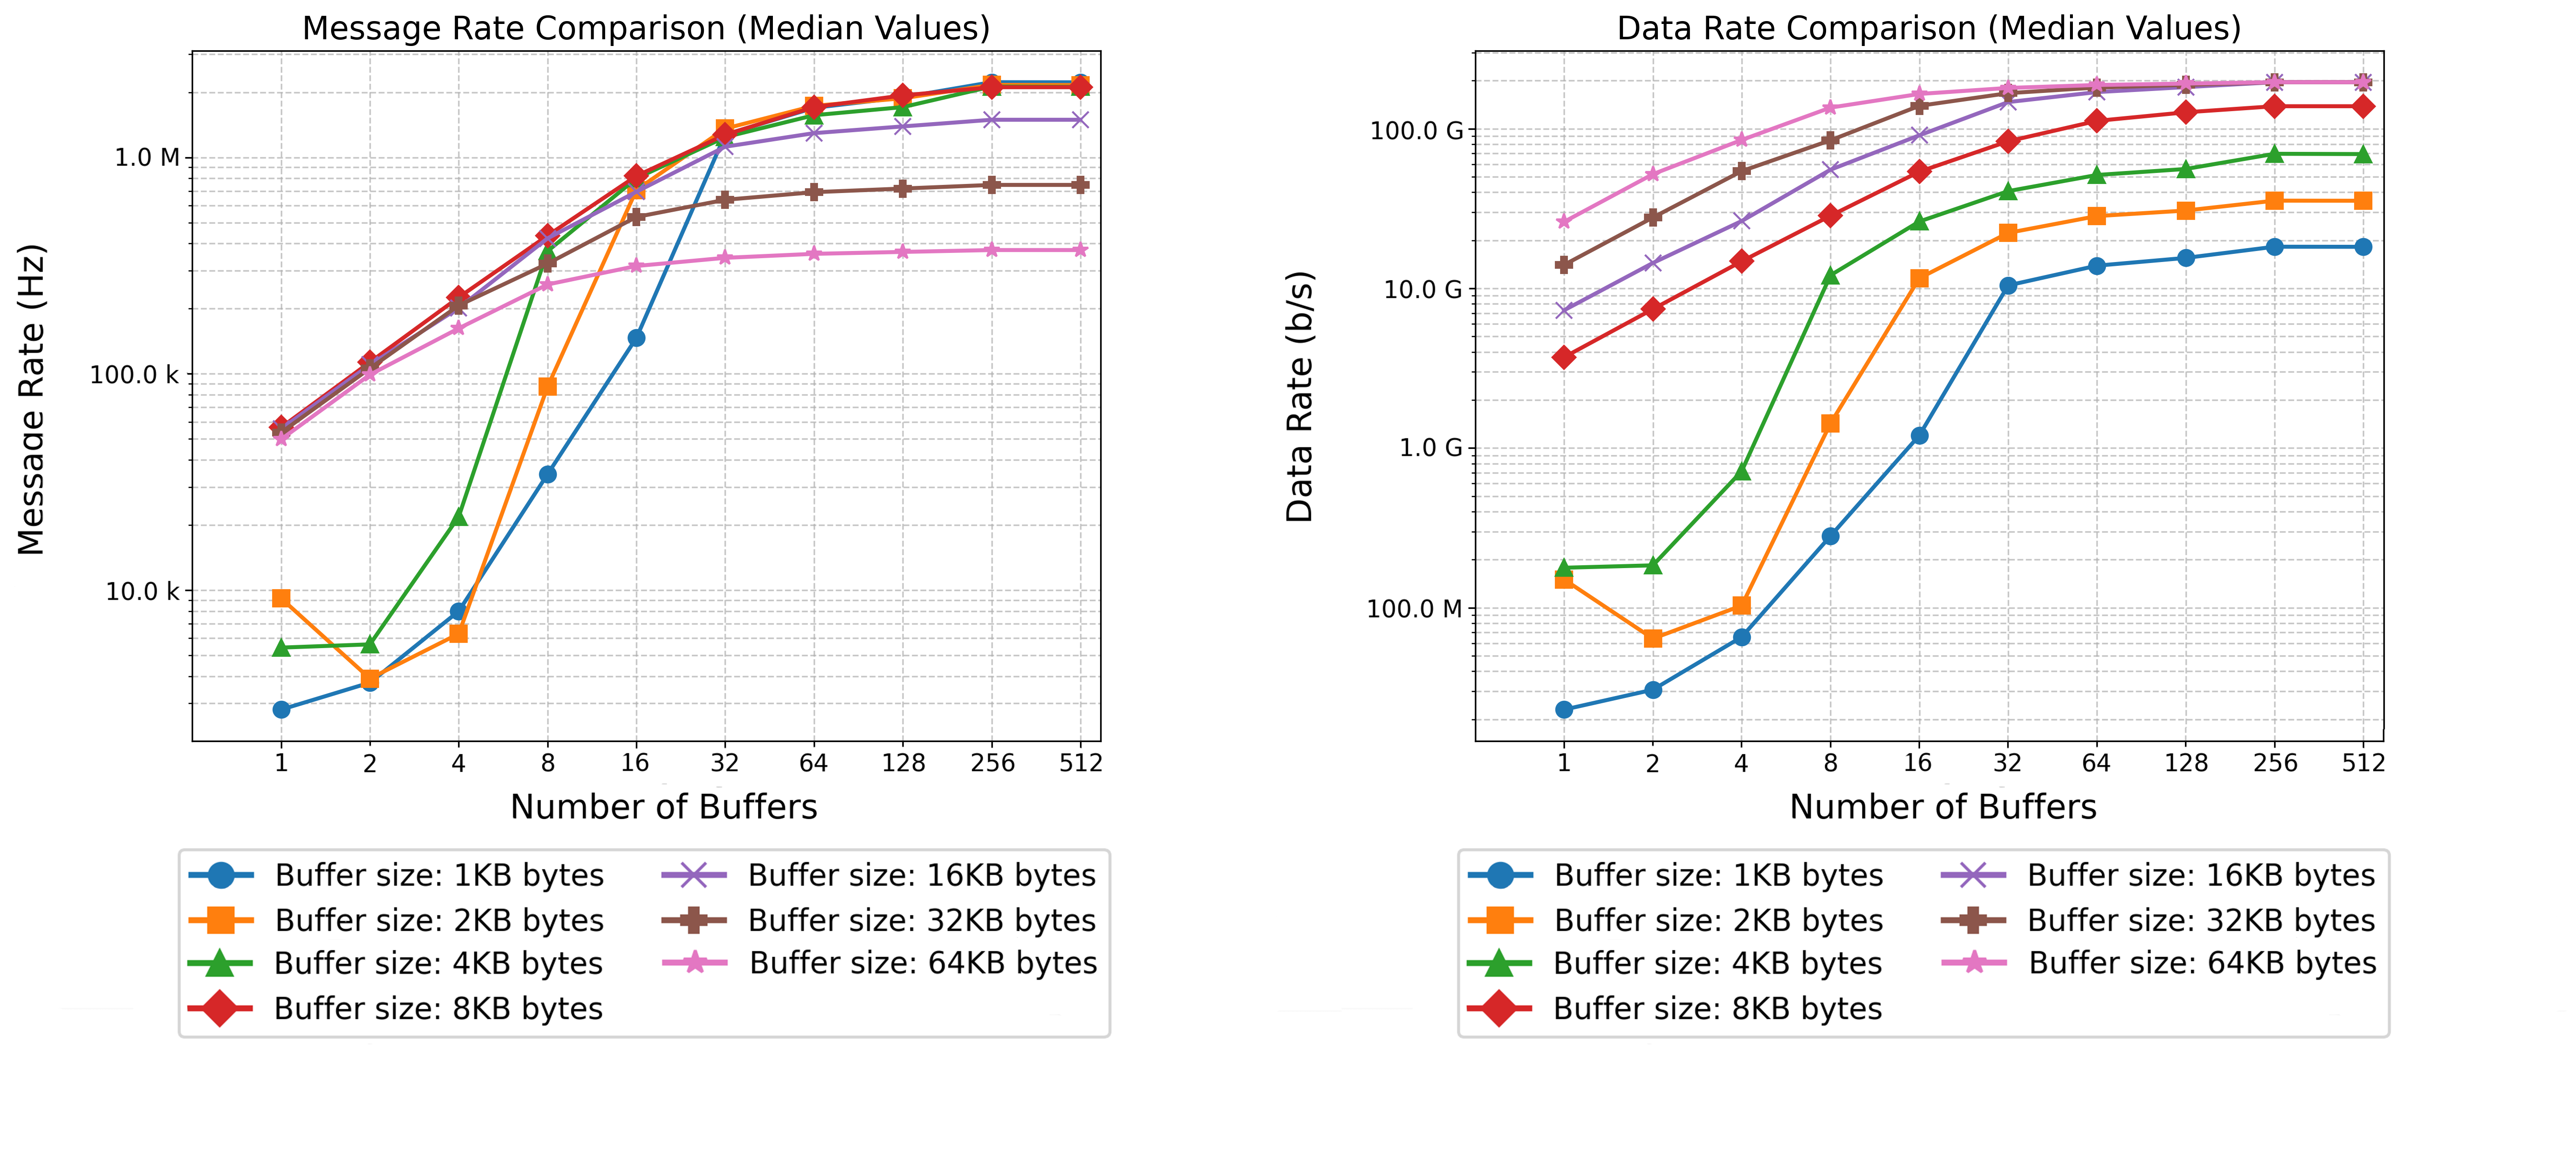
\includegraphics[width=\textwidth]{images/results/libfabric_performance_comparison.png}
\caption[Throughput comparison for LIBFABRIC-RDMA across all buffer sizes]{Throughput comparison for LIBFABRIC-RDMA across all buffer sizes. Left: frequency; Right: throughput.}
\label{fig:libfabric-mean-throughput-comparison}
\end{figure}

The throughput results also demonstrate that the 200 Gbps bandwidth is quickly saturated when using larger buffers. Notably, the network library meets the requirements of 1MHz for Phase II production with a number of buffers \geq 32 and for buffer sizes \leq 16KB (which is far bigger than what will be used at those rates in production).

For ASYNCMSG-TCP, the results (Figure \ref{fig:tcp-mean-throughput-comparison}) reveal that smaller buffers consistently achieve higher rates, regardless of the number of buffers. The throughput is significantly lower than LIBFABRIC-RDMA, with rates ranging from 70 to 90 kHz and a maximum throughput below 10 Gbps. This performance disparity shows once again that LIBFABRIC-RDMA can handle larger amount of data compared to ASYNCMSG-TCP.

\begin{figure}[htbp]
\centering
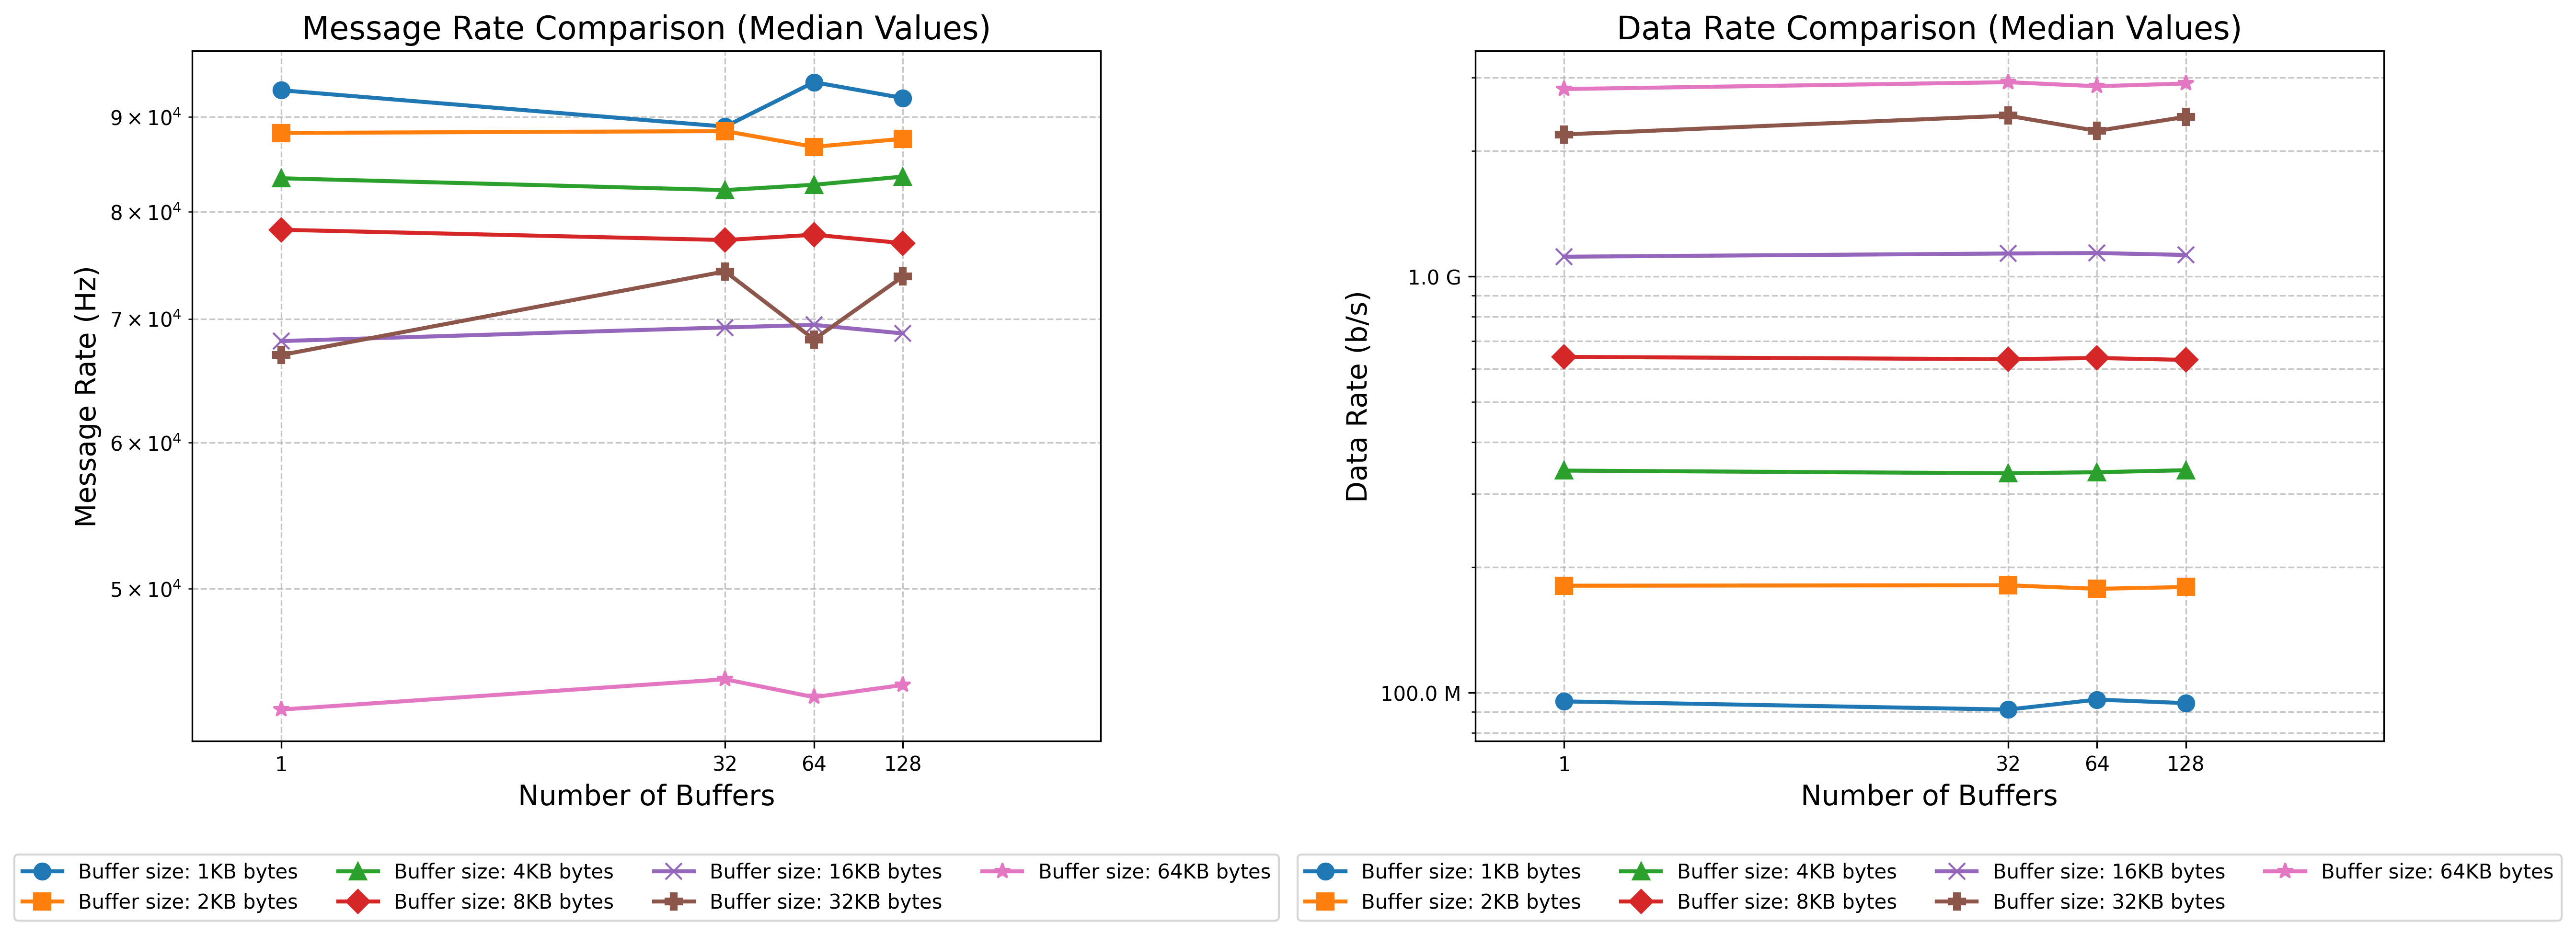
\includegraphics[width=\textwidth]{images/results/tcp_performance_comparison.png}
\caption[Throughput comparison for ASYNCMSG-TCP across all buffer sizes]{Throughput comparison for ASYNCMSG-TCP across all buffer sizes. Left: frequency; Right: throughput.}
\label{fig:tcp-mean-throughput-comparison}
\end{figure}

The decision to limit the number of buffers and sizes tested for ASYNCMSG-TCP was based on the observed saturation of bandwidth for LIBFABRIC-RDMA and the lack of performance improvement for ASYNCMSG-TCP with larger buffers. These findings conclusively demonstrate that LIBFABRIC-RDMA outperforms ASYNCMSG-TCP in terms of data throughput.

Given those results, why is TCP included as an option? There are technical reasons and internal ones. Technically, the pros for TCP over RDMA include simplicity, a smaller memory footprint, opening connections is less costly and, as mentioned before, memory stability during the send operation. 
The internal reasons for using TCP in \acs{ATLAS} derive on how its monitoring works. In order to monitor the entirety of \acs{ATLAS}' \acl{FE} electronics many elinks need to be used, in that case using LIBFABRIC-RDMA would require creating a \acs{DMA} buffer for each of them, plus sometimes the network library is used to send configurations to \acs{FE} electronics, meaning that the buffers need to be big enough for such scenarios. It comes by itself that the amount of memory needed is very large, and that memory would not be used efficiently, also the use case of the monitoring does not require high performance, thus ASYNCMSG-TCP is ideal.

\subsection{\acf{RTT}}

The \acl{RTT} tests were conducted using the two \textit{netio3-backends} LIBFABRIC-RDMA and ASYNCMSG-TCP with the \texttt{epoll} event-loop and \texttt{BOOST::ASIO} event-loop. The test has been manually performed on the two servers previously described using a client and server application developed for the purpose. The output was processed using a custom Python script, which also generated the graphs using the Matplotlib \cite{matplotlib} library. The tests involved sending 25 messages of 64 bytes in size and measuring the \acl{RTT}.

\subsubsection{Analysis}

Figure~\ref{fig:rtt-tcp-rdma} illustrates the average \acs{RTT} of 64-byte messages transmitted using ASYNCMSG-TCP and LIBFABRIC-RDMA backends, with both epoll and BOOST:ASIO event loops. The results show that LIBFABRIC-RDMA achieves significantly lower \acs{RTT} compared to the ASYNCMSG-TCP implementation, regardless of the event loop used. Furthermore using the BOOST:ASIO eventloop consistently outperforms epoll; the reason derives from the implementation of the eventloop, in which the underlying is always \texttt{BOOSt::ASIO}, while the \texttt{epoll} offers a better interface but has to transfer the messages from its thread to the \texttt{BOOST::ASIO} thread.
For ASYNCMSG-TCP, using BOOST:ASIO nearly halves the average \acs{RTT}; the performance increase is noticeable, at the cost of a worse interface and less control.

\begin{figure}[htbp]
\centering
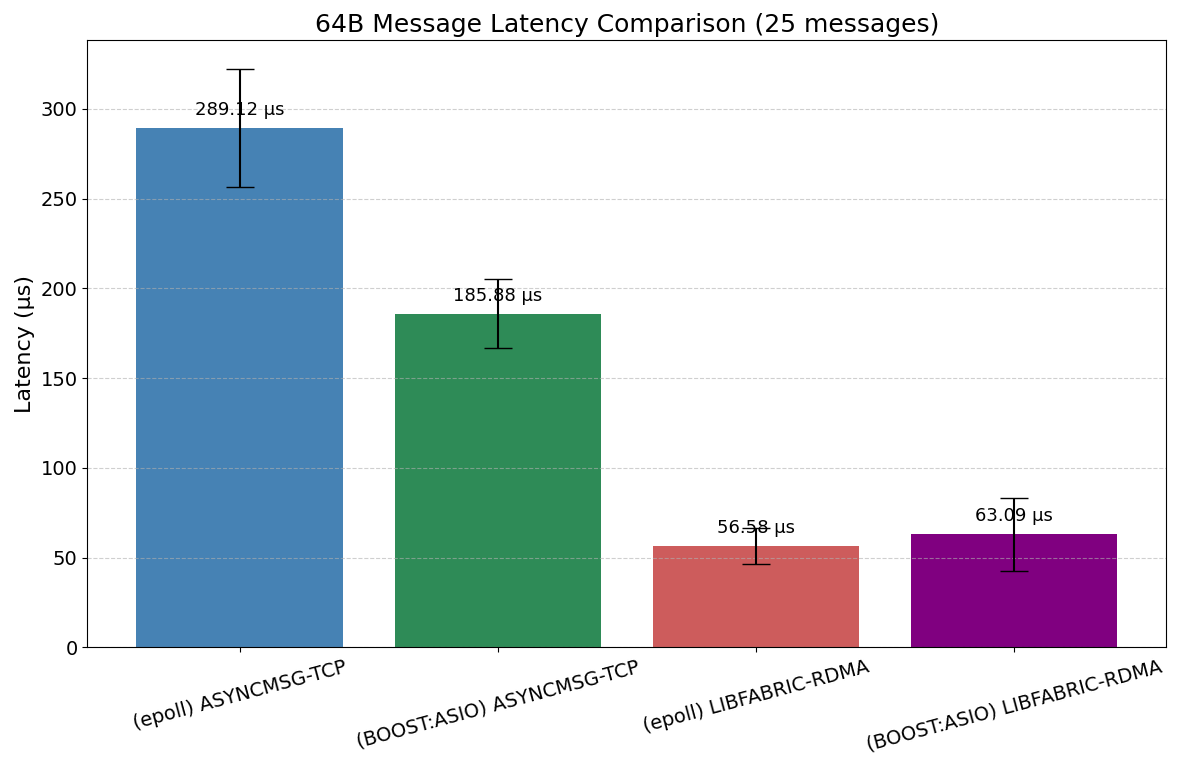
\includegraphics[width=\textwidth]{images/results/rtt.png}
\caption[RTT plot]{RTT plot of ASYNCMSG-TCP and LIBFABRIC-RDMA backends. The unit of measurement is in microseconds.}
\label{fig:rtt-tcp-rdma}
\end{figure}

Table~\ref{tab:rtt-comparison} summarizes the previous analysis.

\begin{table}[ht]
\centering
\begin{tabular}{|l|c|c|}
\hline
\textbf{Setup} & \textbf{Mean (µs)} & \textbf{Std Dev (µs)} \\
\hline
(epoll) ASYNCMSG-TCP & 321.56 & 34.17 \\
(BOOST:ASIO) ASYNCMSG-TCP & 185.88 & 20.40 \\
(epoll) LIBFABRIC-RDMA & 56.58 & 10.31 \\
(BOOST:ASIO) LIBFABRIC-RDMA & 60.45 & 18.91 \\
\hline
\end{tabular}
\caption{RTT comparison for ASYNCMSG-TCP and LIBFABRIC-RDMA.}
\label{tab:rtt-comparison}
\end{table}

LIBFABRIC-RDMA comes with a high connection establishment cost. In the previous analysis the \acs{RTT} of the connection establishment has been considered an outlier and not used in the plot. Figure~\ref{fig:rtt-rdma-outlier} shows the effects of the outlier on the LIBFABRIC-RDMA backend \acs{RTT}. The outliers (323 µs for \texttt{epoll} and 329 µs for \texttt{BOOST::ASIO}) skew the average \acs{RTT} and increase the standard deviation over 25 messages.

\begin{figure}[htbp]
\centering
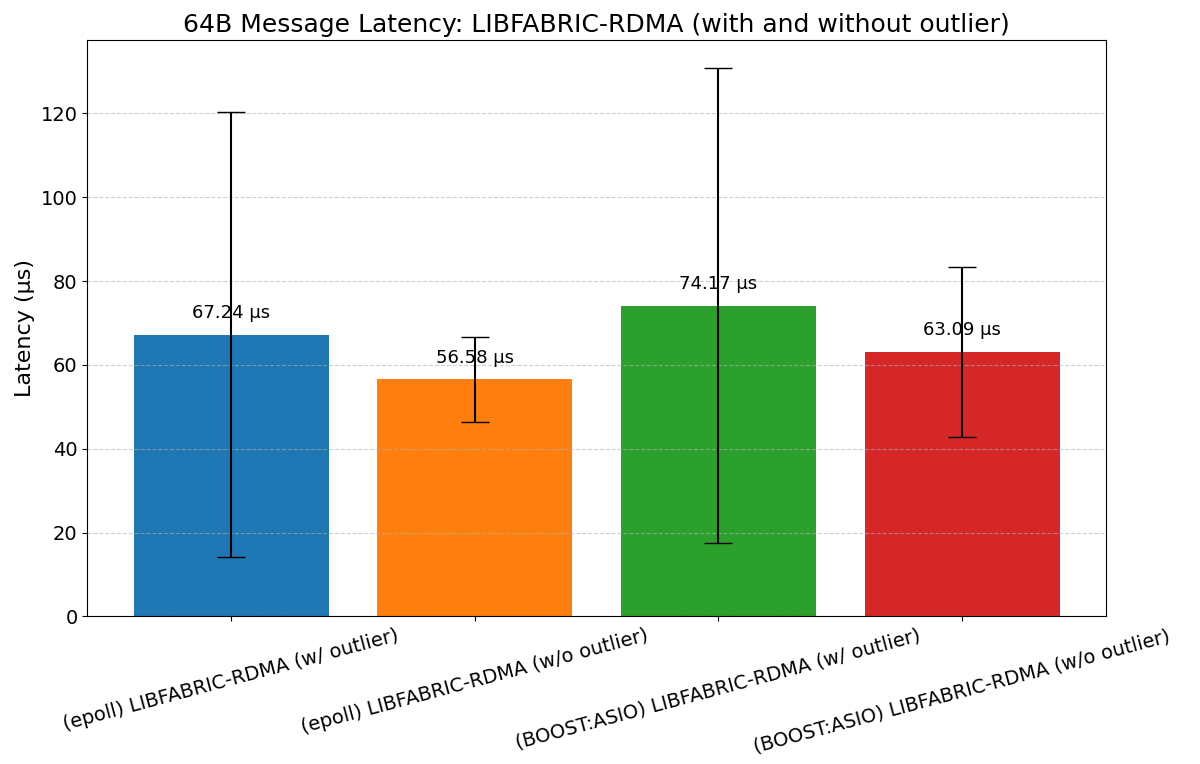
\includegraphics[width=\textwidth]{images/results/rtt-RDMA-outliers.png}
\caption[RDMA RTT plot, with outliers]{RTT plot of LIBFABRIC-RDMA backend with and without the connection establishment outlier. The unit of measurement is in microseconds.}
\label{fig:rtt-rdma-outlier}
\end{figure}

Table~\ref{tab:rtt-outlier} summarizes the previous analysis.

\begin{table}[ht]
\centering
\begin{tabular}{|l|c|c|c|}
\hline
\textbf{Setup} & \textbf{Mean (µs)} & \textbf{Std Dev (µs)} & \textbf{Outlier (µs)} \\
\hline
(epoll) LIBFABRIC-RDMA (w/ outlier) & 67.24 & 43.94 & 323 \\
(epoll) LIBFABRIC-RDMA (w/o outlier) & 56.58 & 10.31 & -- \\
(BOOST:ASIO) LIBFABRIC-RDMA (w/ outlier) & 71.20 & 42.68 & 329 \\
(BOOST:ASIO) LIBFABRIC-RDMA (w/o outlier) & 60.45 & 18.91 & -- \\
\hline
\end{tabular}
\caption{Effect of outlier on LIBFABRIC-RDMA RTT.}
\label{tab:rtt-outlier}
\end{table}

\clearpage
\section{Performance measurements: felix-tohost}

\texttt{felix-tohost} represents the data direction from the Detectors to the T-DAQ infrastructure and between. The measurements that follow were conducted on the same device and host used for the \texttt{netio3} performance evaluation (Section~\ref{sec:netio3-perf}). 
Figure~\ref{fig:tbed-setup} below illustrates the setup for the test.\\
\emph{pc-tbed-felix-15} mounts the currently used in production \emph{FLX-712} with the \emph{F-EMU} firmware, which is used to emulate data in the FULLMODE format; that data is written inside \acs{DMA} buffers on the other machine through \acs{E-link}s. It can be configured which \acs{E-link} writes in which \acs{DMA} buffer using the \emph{elinkconfig} tool. In the context of this test, all the 12 links have been used, specifically 3 links per \acs{DMA} buffer. 
On the same machine runs \emph{felix-test-swrod}, which is a software that subscribes to the \acs{E-link}s through \texttt{felix-tohost}, which in turn publishes the data when available.
On \emph{pc-tbed-felix-14} is mounted an \emph{FLX-182-1B} card, with FULLMODE firmware. On the machine runs \texttt{felix-tohost}, which, as mentioned, publishes the data received from the emulator to \emph{felix-test-swrod} and posts the monitoring data so that a Prometheus instance running on Docker on my local machine could scrape it, and in turn Grafana could query Prometheus for the data scraped and create the Dashboard seen in Figure~\ref{fig:tohost-perf}. On \emph{pc-tbed-felix-14}, there is also the \acl{TTC} emulator that gives the pace to the FULLMODE emulator; in this test, the emulator trigger signals were set at 1 MHz.\\
For what concerns the \emph{netio3} network library, LIBFABRIC-RDMA was used.\\
The test consisted of sending data through all 12 links distributed across 4 \acs{DMA} buffers (3 links per \acs{DMA} buffer) at a steady 1 MHz rate, but changing the \emph{chunk} size. For reading each DMA buffer have been used 3 threads.\\
It is relavant to introduce a technical firmware implementation of the \acs{FELIX} card; When a \acs{FELIX} card is inserted into the PCIe socket, it presents itself as two PCIe endpoints, which to the Operating System appear as separate devices; this is useful because each device can have its own DMA buffer and control logic. For the test \texttt{felix-tohost} has been run using two devices presented by the FLX-182.\\
As a reminder, in FULL mode, each link is not subdivided into \acs{E-link}s.

\begin{figure}[htbp]
\centering
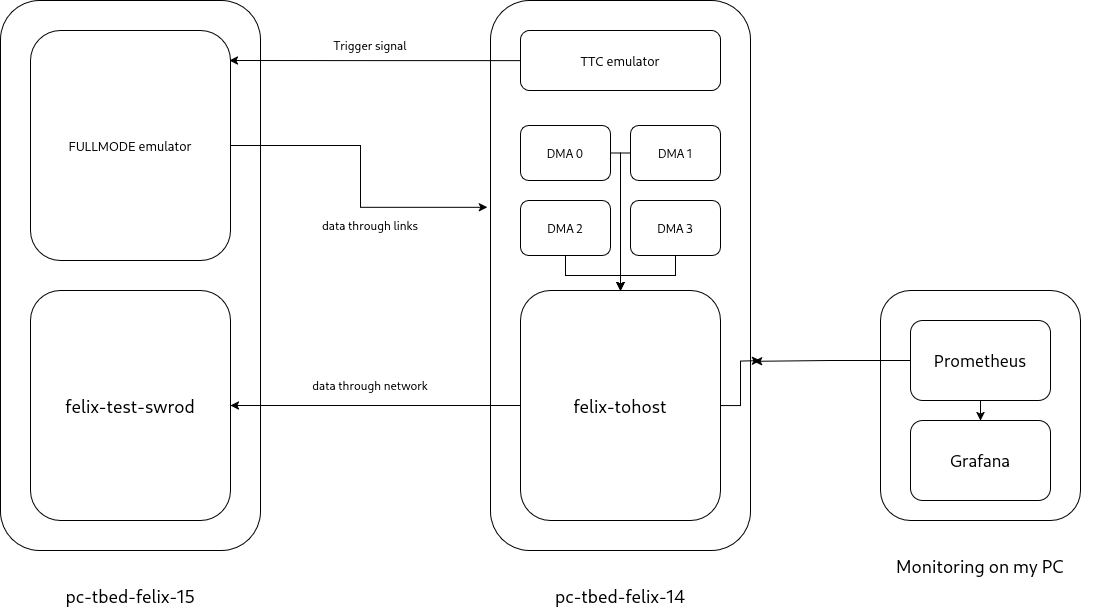
\includegraphics[width=\textwidth]{images/results/tohost-tbed-setup.png}
\caption[Testbed configuration]{Testbed configuration. F-EMU firmware is installed on the felix-15 machine, felix-tohost is running on the felix-14 machine which also sends the monitoring data to Prometheus.}
\label{fig:tbed-setup}
\end{figure}

The monitoring system described in Section~\ref{sec:felix_monitoring} was employed to record the performance evaluation, in particular the Prometheus-Grafana solution. The test was conducted by gradually increasing the \emph{chunk} size while maintaining a steady rate of 1 MHz (that is the requirement for Phase II). This behavior is illustrated in the dashboard window titled "Average Chunk Size" (Image~\ref{fig:tohost-perf}), where the average chunk size ramps, with incremental steps, from 16 bytes to 2 KB. Starting at a chunk size of 1 KB, by looking at the \emph{E-link Chunk Rate} graph it appears that performance issues begin to arise.\\
What in reality is shown in the image is not a performance issue, but it is the reach of the physiological limit of FULL mode. To recall, the Subsection~\ref{subsec:felix-fullmode} explains that FULL mode has a maximum theoretical throughput of about 7.68 Gbps per link (after encoding, which is our case), and in the graph it is shown that the \acs{DMA} buffers are not getting filled up (\emph{Free Space in DMA Buffer} graph), there is no backpressure in the network (\emph{Network Resources} graph) and the chunks are not being truncated (\emph{Chunks Truncated} graphs). at a rate of 1MHz, sending 1KB of data per chunk means that the throughput is about 8.2 Gbps, and at 2KB it is about 16.4 Gbps, which is above the maximum throughput of the link, thus the link chunk rate diminishes untill reaching 7.68 Gbps throughput.\\ 
To recap, in figure~\ref{fig:tohost-perf} is shown that \texttt{felix-tohost} and the card \texttt{FLX-182-1B} can handle without signs of distress data rates that reach the technological limit of FULL mode.

\begin{figure}[htbp]
\centering
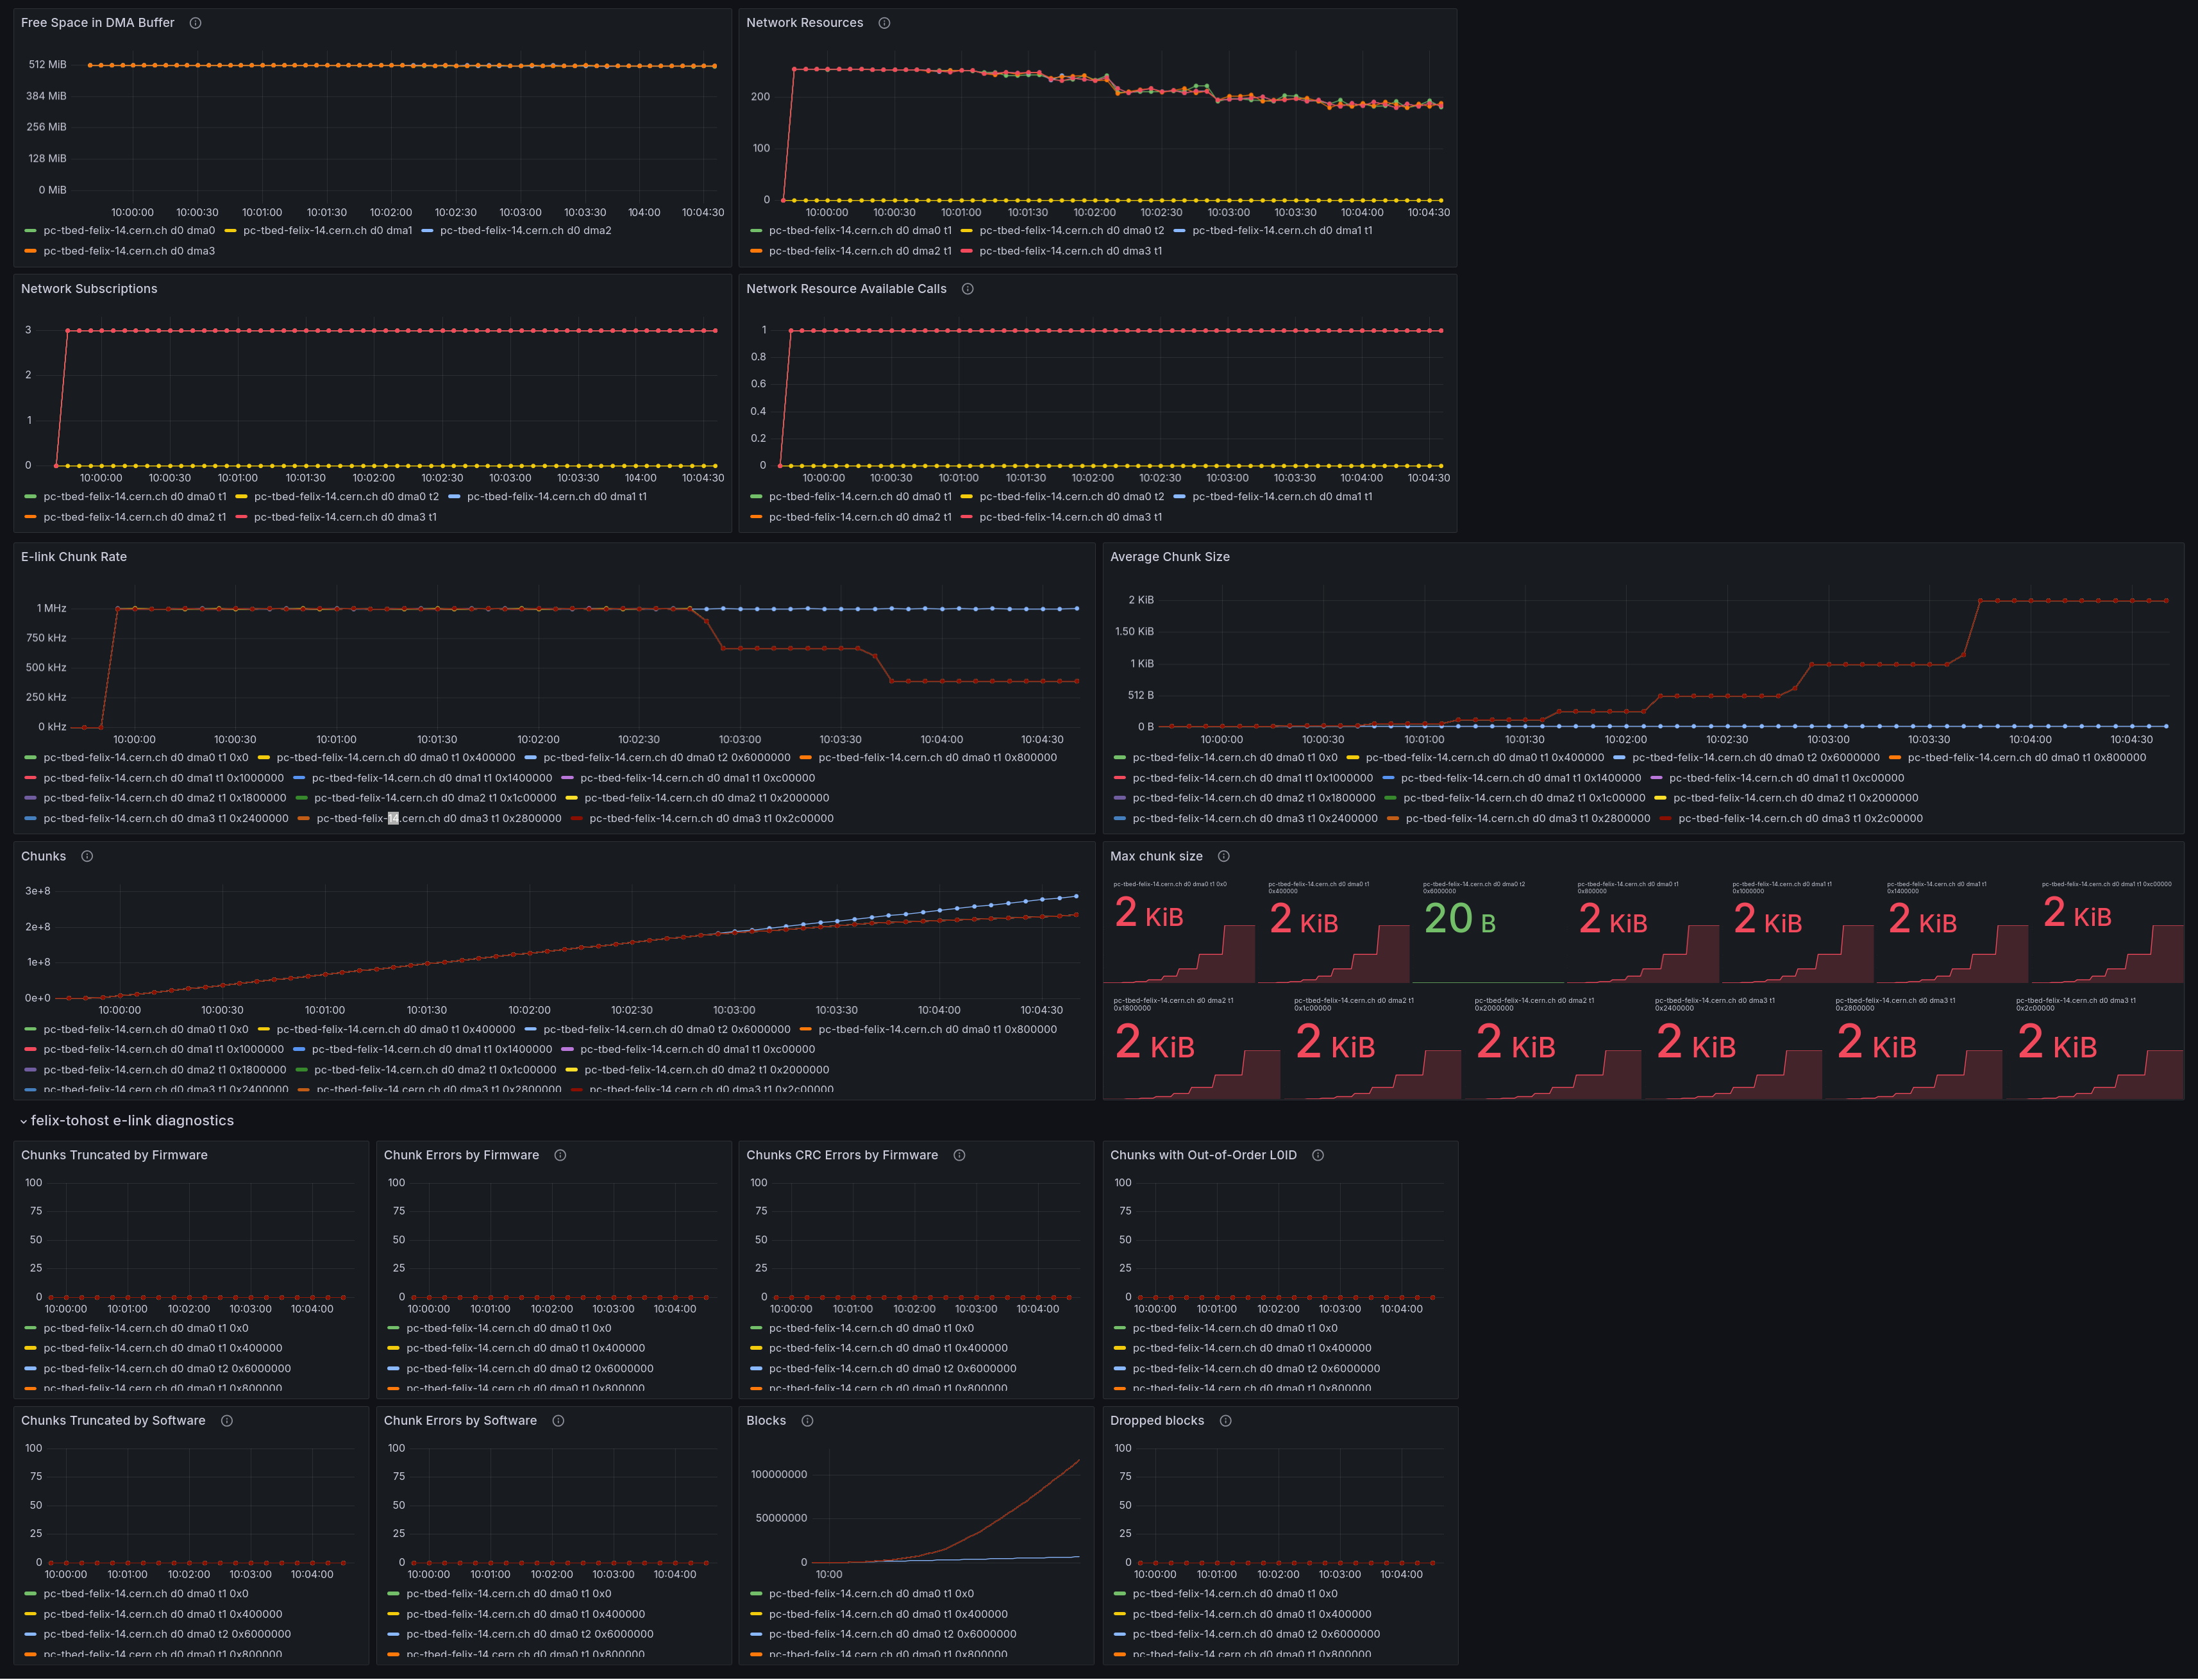
\includegraphics[width=\textwidth]{images/results/tohost-perf.png}
\caption{Grafana monitoring: stress test at 1 MHz rate up to 2 KB chunks.}
\label{fig:tohost-perf}
\end{figure}

Figure~\ref{fig:cpu-usage} illustrates the CPU usage per chunk size. The percentage value represents the average CPU usage over a 30-second period. 760 bytes chunk size is around the theoretical maximum that FULL mode can handle; the CPU usage with 760 bytes sized messages is about 700\%; There are two \acs{FELIX} cards mounted on a server, thus doubling the total CPU requirements; this brings to the conclusion that the host machine must have a minimum of 14 cores in order to run \emph{felix-tohost} with the theoretical maximum chunk size at a 1MHz rate.

\begin{figure}[htbp]
\centering
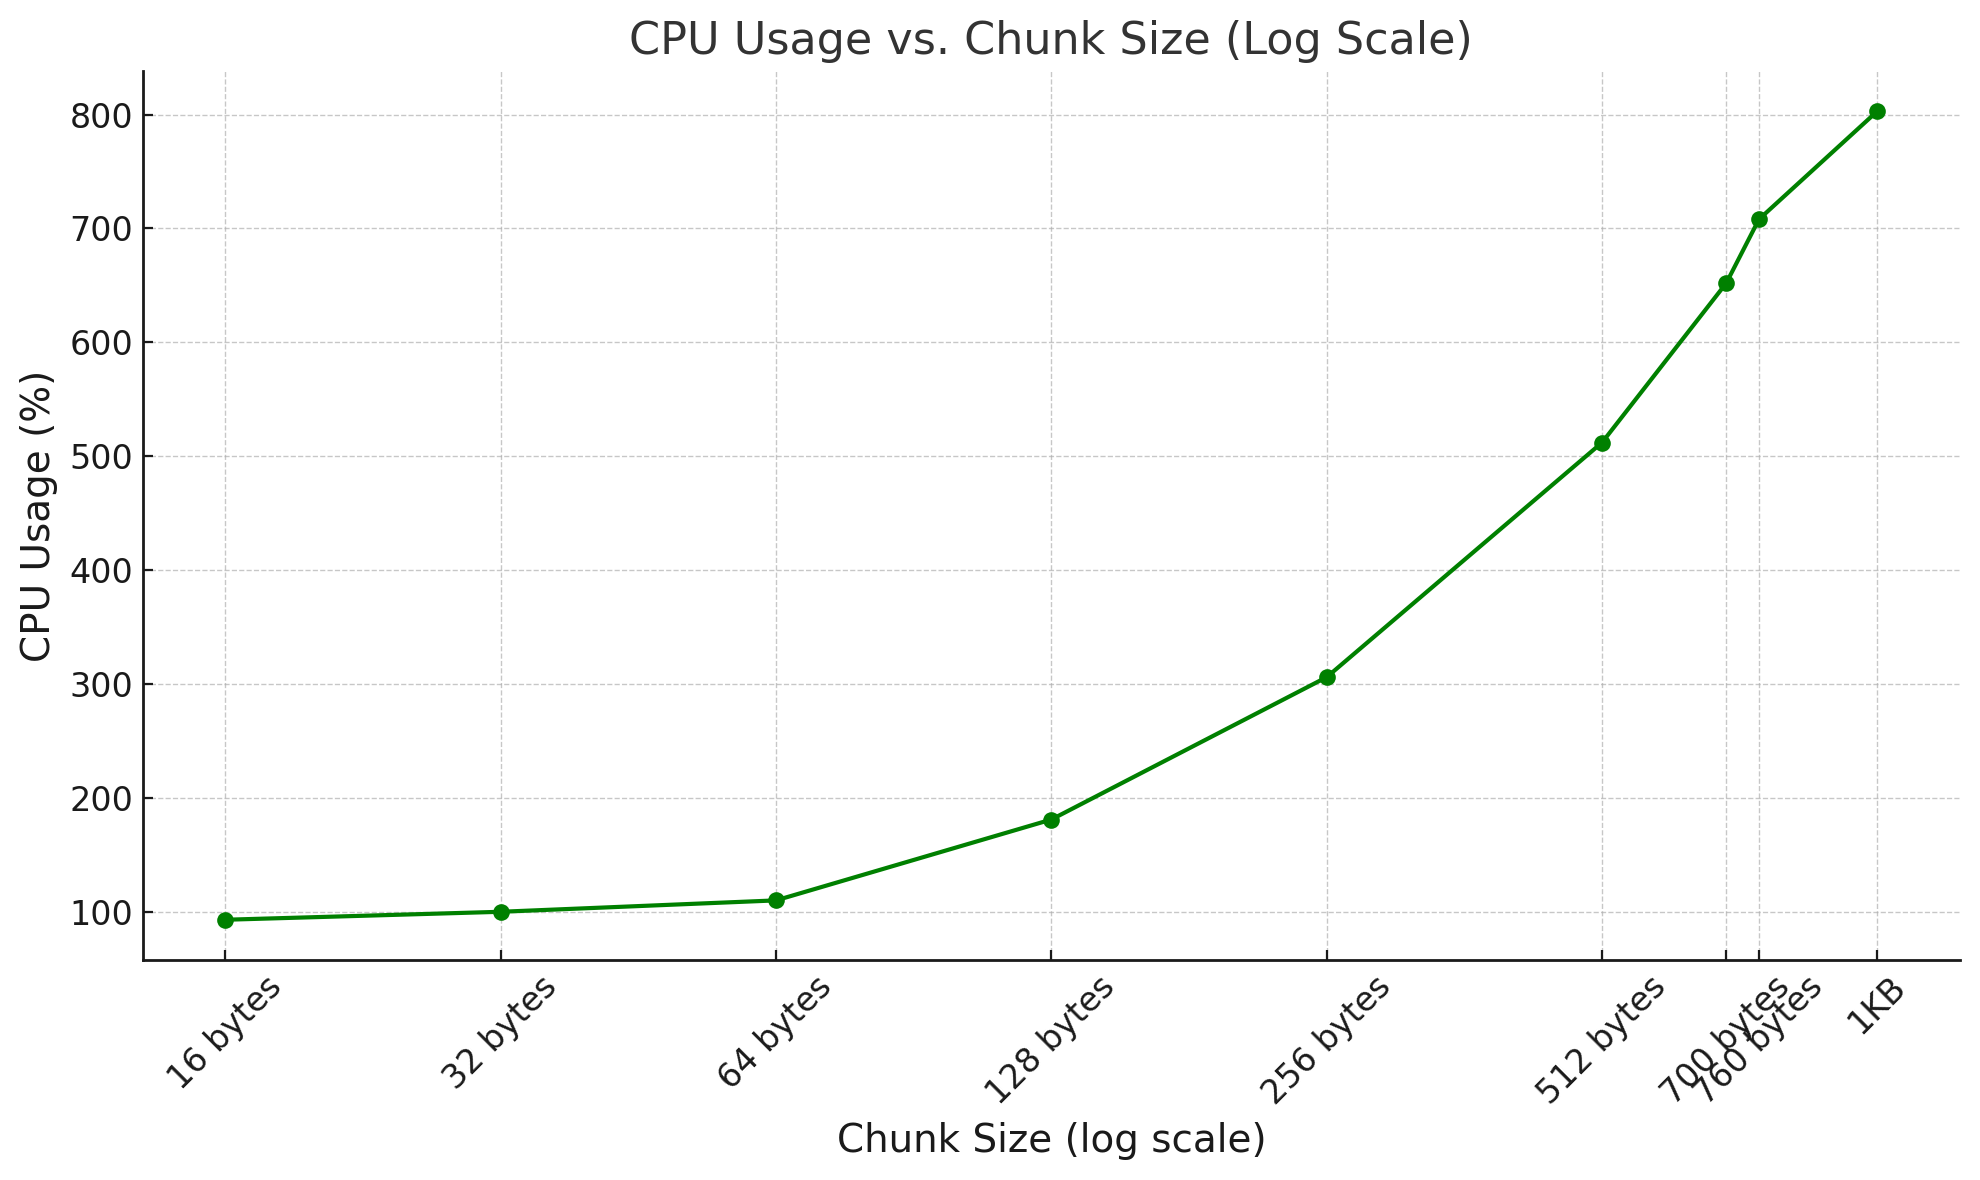
\includegraphics[width=\textwidth]{images/results/cpu-usage-chunk-size-1MHz.png}
\caption[CPU usage per chunk size at 1 MHz]{CPU usage per chunk size at 1 MHz. 100\% corresponds to one physical CPU core.}
\label{fig:cpu-usage}
\end{figure}

The execution of \texttt{felix-tohost} was analyzed using \texttt{perf}, and from the output a FlameGraph \cite{flamegraph} was generated (Figure~\ref{fig:felix-tohost-flamegraph}). The FlameGraph, an interactive \emph{svg} file viewable in a web browser, shows that a significant portion of the execution time is spent on functions such as \emph{decode\_subchunk\_headers}, \emph{post\_subchunk}, and \emph{check\_block\_integrity}, as well as chunk-copying operations. This flamegraph shows hotpost areas in the code that can potentially be optimized, serving as a starting point for future developments (see Subsection~\ref{subsec:felix-tohost-improvement}).

\begin{figure}[htbp]
\centering
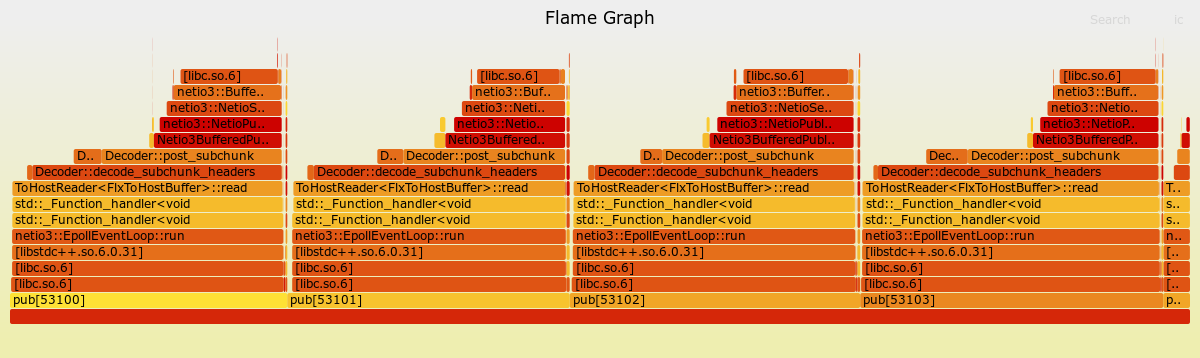
\includegraphics[width=\textwidth]{images/results/flamegraph.png}
\caption[Flamegraph of felix-tohost]{Flamegraph of \texttt{felix-tohost} reading from one device. It highlights four main processes, each corresponding to one \acs{DMA} buffer, along with a smaller fifth process dedicated to \acs{TTC}.}\label{fig:felix-tohost-flamegraph}
\end{figure}